\subsection{Poisson Equation}
\label{ssec:result_green}

% {\bf The main points to get across here are: (i) that with a specific
% reduction of the architecture we recover Green's function;
% (ii) that we can learn something that is independent of the
% measure used for training (generalization). I think the results
% we have in 1D and 2D need to be improved. It is possible to show
% that an increasingly rich parameterization leads to better
% results?}\\

% {\bf the figures are to be replaced}\\

% {\bf fix the scale, use better color }\\

\iffalse
First, as a illustration, we want to show with a specific
reduction of the architecture we recover Green's function.
We use the 1d poisson equation defined in section   \ref{ssec:poisson} as the test function, because it is simple enough to have an analytic Green function, and also because in the 1d case, we can visualize the kernel as a 2d image. As discussed in section \ref{ssec:poisson}, the true Green function has the form:
\[G(x,y) = \frac{1}{2} \left ( x + y - |y-x| \right ) - xy. \]
so that $u(x)  = \int_0^1 G(x,y) f(y) \mathrm{d}y$.  It is visualized on the right of Figure \ref{fig:kernel1d_nystrom}.

Again, for this problem,
we consider a simplification of the iterative update framework defined in section \ref{sec:framework}. We omit step 1.,2. and 4. and only use one iteration of step 3. In other words, we set \(v_0(x) = f(x)\), \(T=1\), \(n=1\), \(\sigma(x) = x\), \(W = w = 0\), and \(\nu_x(dy) = dy\) (the Lebesgue measure). The purposed operator $\cF$ can be directly written as
\[(\cF f)(x) = \int_0^1 \kappa(x,y; \phi) f(y) \mathrm{d}y \]
For this test problem, we want to show whether the neural network $\kappa$ will match the Green function $G$.
\fi

Recall the Poisson equation \eqref{eq:poisson} introduced in subsection~\ref{ssec:poisson}. We use a zero hidden layer neural operator construction without lifting the input dimension. In particular, we simply learn a kernel \(\kappa_\theta : \R^2 \to \R\) parameterized as a standard feed-forward neural network with parameters \(\theta\). Using only \(N = 1000\)
training examples, we obtain a relative test error of \(10^{-7}\). The neural operator gives an almost perfect approximation to the true solution operator in the topology of \eqref{eq:bochner_error}.

To examine the quality of the approximation in the much stronger uniform topology, we check whether the kernel \(\kappa_\theta\) approximates the Green's function for this problem. To see why this is enough, let \(K \subset L^2([0,1];\R)\) be a bounded set i.e.
\[\|f\|_{L^2([0,1];\R)} \leq M, \qquad \forall f \in K\]
and suppose that
\[\sup_{(x,y) \in [0,1]^2} |\kappa_\theta(x,y) - G(x,y)| < \frac{\epsilon}{M}.\]
for some \(\epsilon > 0\). Then it is easy to see that
\[\sup_{f \in K} \|\Ftrue (f) - \G_\theta (f)\|_{L^2([0,1];\R)} < \epsilon,\]
in particular, we obtain an approximation in the topology of uniform convergence over bounded sets, while having trained only in the topology of the Bochner norm \eqref{eq:bochner_error}. Figure~\ref{fig:kernel1d_nystrom} shows the results from which we can see that \(\kappa_\theta\) does indeed approximate the Green's function well. This result implies that by constructing a suitable architecture, we can generalize to the entire space and data that is well outside the support of the training set.




% A summary of performance of the four methods on the Poisson equation is listed in the following:
% \begin{itemize}
% \item Nystr\"om:     $1\mathrm{e}{-7}$  
% \item Low-rank:     $r=1$, $1\mathrm{e}{-3}$; $r=10$, $5\mathrm{e}{-7}$; $r=100$, $1\mathrm{e}{-7}$; $r=1000$, $5\mathrm{e}{-8}$
% \item Multipole:     $5\mathrm{e}{-5}$  
% \item Fourier :    $7\mathrm{e}{-4}$ 
% \end{itemize}

% \iffalse
% \begin{table}[h]
% \caption{Error of different methods {\bf shall use relative error}}
% \label{table:green}
% \begin{center}
% \begin{tabular}{l|llll}
% \multicolumn{1}{c}{\bf Methods} 
% &\multicolumn{1}{c}{\bf Error }
% &\multicolumn{1}{c}{\bf } 
% &\multicolumn{1}{c}{\bf }
% &\multicolumn{1}{c}{\bf }\\
% \hline 
% Nystr\"om     &$1\mathrm{e}{-7}$  &  &  &\\
% Low-rank     &$r=1$, $1\mathrm{e}{-3}$ &$r=10$, $5\mathrm{e}{-7}$  &$r=100$, $1\mathrm{e}{-7}$ &$r=1000$, $5\mathrm{e}{-8}$\\
% Multipole     &$5\mathrm{e}{-5}$  &  & &\\
% Fourier     &$7\mathrm{e}{-4}$ & & &\\
% \hline 
% \end{tabular}
% \end{center}
% \end{table}
% \fi

% \subsubsection{Nystrom approximation method}
\begin{figure}[t]
    \centering
    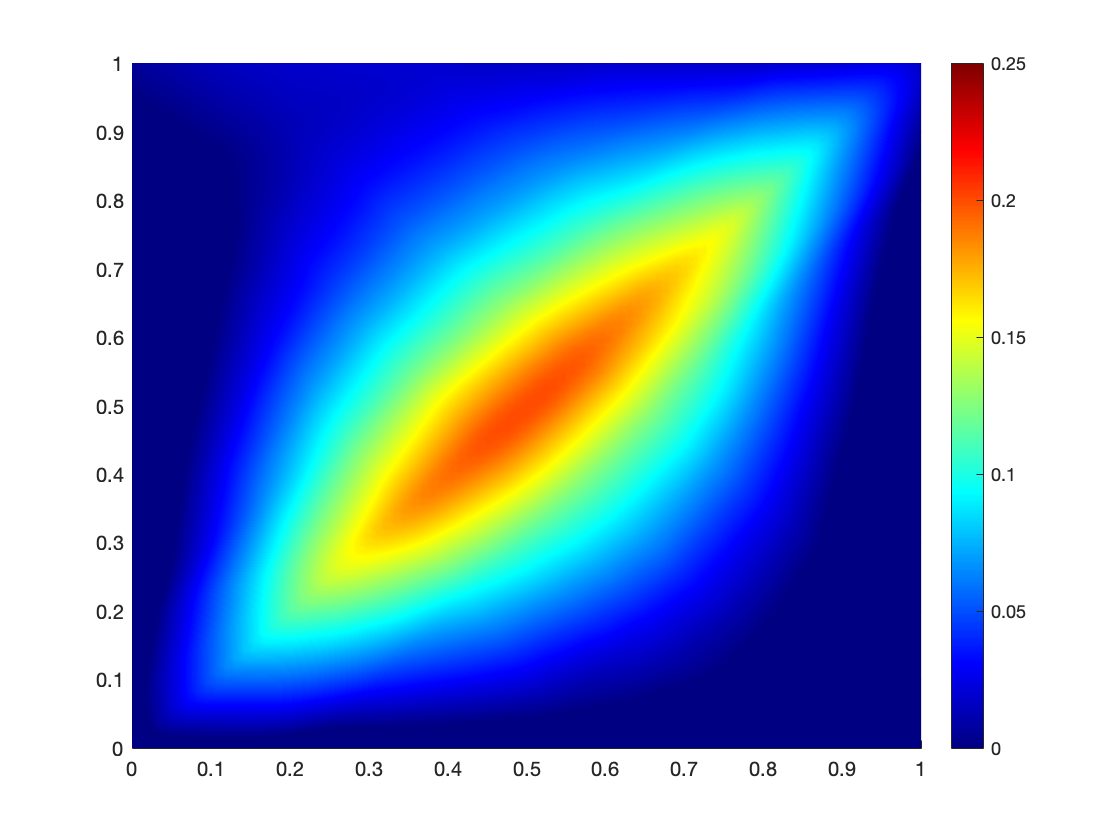
\includegraphics[width=0.48\textwidth]{Figs/greens_pred.png}
    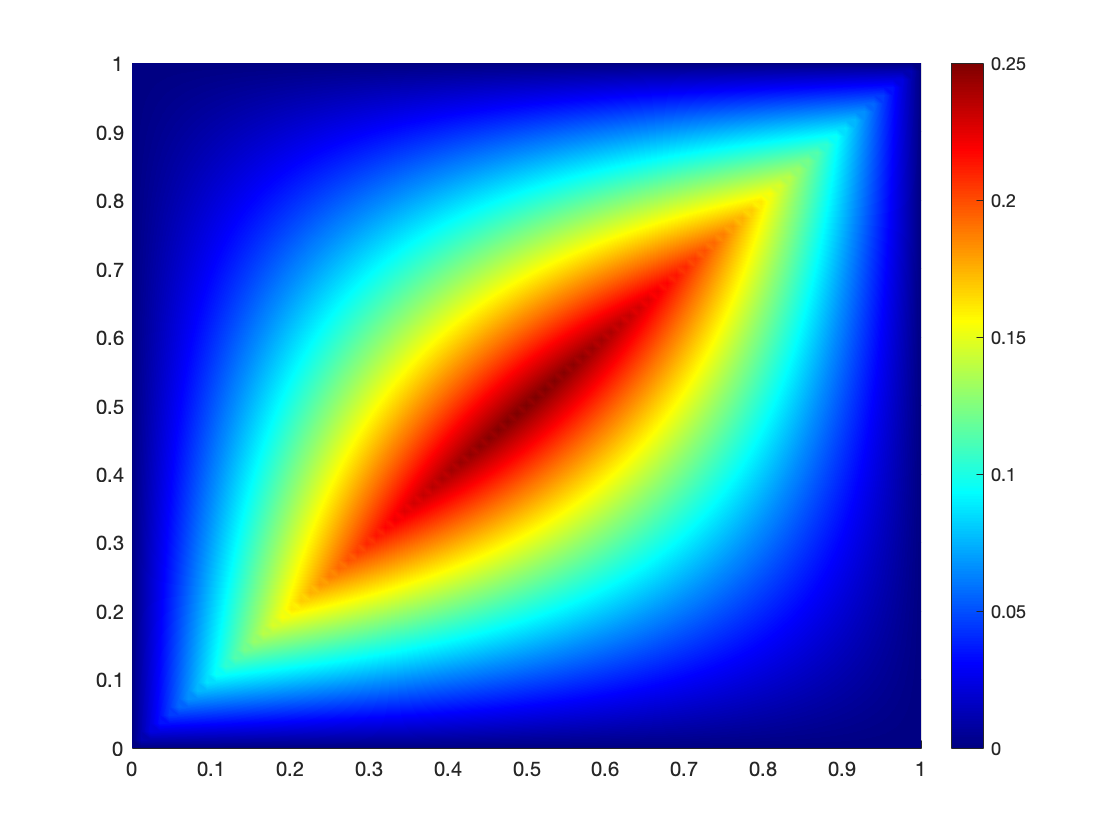
\includegraphics[width=0.48\textwidth]{Figs/greens_truth.png}
        \caption{Kernel for one-dimensional Green's function, with the Nystrom approximation method}
    \label{fig:kernel1d_nystrom}
    \small{
    {\bf left:} learned kernel function; {\bf right:} the analytic Green's function.\\
    This is a proof of concept of the graph kernel network on $1$ dimensional Poisson equation and the comparison
    of learned and truth kernel.
    }
\end{figure}

\iffalse
The Nystr\"om approximation method has an test error rate of $1\mathrm{e}{-7}$ ({\bf shall use relative error}). As shown in Figure \ref{fig:kernel1d_nystrom}, the learned kernel function $\kappa(x,y)$ is very close to the true Green function $G$. It can be seems that the learned kernel is ``shallower'' and ``wider'' compared to the true Green's function ($\kappa(0.5, 0.5) \approx 0.22$, $G(0.5, 0.5)=0.25$). Because the learn kernel has near zero test error, it implies the learned ``shallower'' and ``wider'' is also a near optimal solution for this equation. It can be seems, the neural networks kernel well approximated the true kernel (the Green's function).
\fi


% \subsubsection{Low rank method}
% \begin{figure}[h]
%     \centering
%  \includegraphics[width=6cm]{Figs/green/s11_lowrank_1.eps}
% \includegraphics[width=6cm]{Figs/green/s11_lowrank_10.eps}\\
% \includegraphics[width=6cm]{Figs/green/s11_lowrank_100.eps}
% \includegraphics[width=6cm]{Figs/green/s11_lowrank_1000.eps}\\
% \small{ {\bf Top left:} rank $1$.  {\bf top right:} rank $10$. {\bf bottom left:} rank $100$. {\bf bottom right:} rank $1000$.  
% }
% \caption{Kernel for one-dimensional Green's function, with the low rank method, {\bf The figures are to be replaced}}
% \label{fig:kernel1d_lowrank}
% \end{figure}
% For the low-rank methods, we impose the low-rank decomposition $\kappa(x,y) = \sum^r_{j=1} \varphi^{(j)}(x) \psi^{(j)}(y)$. We choose the rank to be ${1, 10, 100, 1000}$. Because the poisson equation is and a grid of resolution $85$. The underlying discretized kernel matrix is $85$ by $85$, so it has rank $85$ at most. For $r=1$ or $10$ the low-rank kernel has lower rank than the true discretrized kernel; for $r=100, 1000$, the low-rank kernel has sufficient number of rank.

% It turns out that for $r=1,10,100,1000$, the low-rank method has error $1\mathrm{e}{-3}$,$5\mathrm{e}{-7}$,$1\mathrm{e}{-7}$,$5mathrm{e}{-8}$({\bf shall use relative error}). It can be seen that for $r\geq 10$, the rank is already sufficient. 
% This is visrualized in Figure \ref{fig:kernel1d_lowrank}.  


% \subsubsection{multipole method}
% \begin{figure}[h]
%     \centering
% \includegraphics[width=6cm]{Figs/green/s11_multipole1.eps}
% \includegraphics[width=6cm]{Figs/green/s11_multipole2.eps}
% \includegraphics[width=6cm]{Figs/green/s11_multipole3.eps}\\
% \small{
% }
% \caption{{\bf also include the sum of the three} {\bf The figures are to be replaced}}
% \label{fig:kernel1d_multipole}
% \end{figure}

% \subsubsection{fourier method}
% {\bf The fourier method is ill-posed on this problem. We shall not show that }
% \begin{figure}[h]
%     \centering
%     \includegraphics[width=6cm]{Figs/green/s11_fourier.eps}
% \small{
% }
% \caption{{\bf The figures are to be replaced}}
% \label{fig:kernel1d_fourier}
% \end{figure}